
\chapter{Angular Convolution, A Better Algorithm\label{chpt:angular-convolution}}

In section \ref{chpt:fft-spatial}, the spatial convolution is treated
by FFT thanks to the transitional invariance that leads to $\mathbf{r_{12}}=\mathbf{r_{1}}-\mathbf{r_{2}}$.
However, as the angular grid is not homogeneous, the relative coordinates
of two angles cannot be simply represented $\mathbf{\Omega_{12}}=\mathbf{\Omega_{1}}-\mathbf{\Omega_{2}}$,
therefore we cannot take advantage of the convolution property shown
in eq. (\ref{eq:convolution-1}-\ref{eq:convolution-2}). In other
hand, these two-particle quantities also have rotational invariance.
Proposed by Blum \citep{Blum_I,Blum_II} and used by Fries and Patey
\citep{Fries_Patey_1985}, a rotational invariant expansion technic
reduces the molecular Ornstein-Zernike (MOZ) equation into smaller
irreducible matrix equations. As there is an mathematical equivalence
between IEM and MDFT (section \ref{chpt:mdft}), where eq. (\ref{eq:gamma-k})
can be regarded as the molecular OZ equation, this formalism can be
also applied to MDFT.


\section{Angular convolution using Blum's reduction}

To build a relation between the irreducible form of the molecular
OZ equation deduced by Blum (detailed in section \ref{chpt:iem})
\marginpar{Here the projections $F_{\mu\nu,\chi}^{mn}$ is defined as eq. (appendix)
with symmetries eq. (appendix).\textcolor{red}{{} It's mathematically
identical with {[}ref{]} but using $R_{\mu'\mu}^{m}=D_{\mu'\mu}^{m*}$.}} 
\begin{equation}
\hat{\gamma'}_{\lambda\mu,\chi}^{lm}(k)=\sum_{n=0}^{n_{\mathrm{max}}}\sum_{\nu=-n}^{n}\left(-\right){}^{\chi+\nu}\Delta\hat{\rho'}_{\lambda\underline{\nu},\chi}^{ln}(k)\hat{c'}_{\mu\nu,\chi}^{mn}(k)\label{eq:Blum-reduced-OZ}
\end{equation}
and the MDFT, a generalized spherical harmonic transform (GSHT) treatment
is proposed by Luc Belloni, developing the functional gradient $\hat{\gamma}$
and the density $\hat{\rho}$ in eq. (\ref{eq:gamma-k}) on Wigner
generalized spherical harmonics (GSH):
\begin{equation}
\hat{\gamma}(\mathbf{k},\mathbf{\Omega_{1}})=\sum_{m\mu'\mu}f_{m}\hat{\gamma}_{\mu'\mu}^{m}(\mathbf{k})R_{\mu'\mu}^{m}(\mathbf{\Omega_{1}})\label{eq:gamma-projection}
\end{equation}
\begin{equation}
\Delta\hat{\rho}(\mathbf{k},\mathbf{\Omega_{2}})=\sum_{n\nu'\nu}f_{n}\Delta\hat{\rho}_{\nu',\nu}^{n}(\mathbf{k})R_{\nu',\nu}^{n}(\mathbf{\Omega_{2}})\label{eq:delta-rho-projection}
\end{equation}
where $0\leq m\leq m_{\mathrm{max}}$, $\left|\mu'\right|,\left|\mu\right|<m$
and $\left|\nu'\right|,\left|\nu\right|<n$. $f_{m}=\left(2m+1\right)^{\frac{1}{2}}$
is the normalization factor (according to Luc's definition).

The DCF can also be expended on rotational invariants \citep{Blum_I},
with the normalization factors according to Luc's definition:
\begin{equation}
\hat{c}(k,\mathbf{\Omega_{1}},\mathbf{\Omega_{2}})=\sum_{mnl\mu\nu}f_{m}f_{n}\hat{c}_{\mu\nu}^{mnl}(k)\sum_{\mu'\nu'\lambda'}\left(\begin{array}{ccc}
m & n & l\\
\mu' & \nu' & \lambda'
\end{array}\right)R_{\mu'\mu}^{m}(\mathbf{\Omega_{1}})R_{\nu'\nu}^{n}(\mathbf{\Omega_{2}})R_{\lambda'0}^{l}(\hat{\mathbf{k}})\label{eq:c-projection}
\end{equation}


As GSH possess orthogonality eq. (\ref{eq:gsh-orthogonality}) and
symmetry eq. (\ref{eq:symm-gsh-1}), eq. (\ref{eq:gamma-k}) can be
rewritten by (\ref{eq:gamma-projection}, \ref{eq:delta-rho-projection},
\ref{eq:c-projection}), which gives
\begin{equation}
\hat{\gamma}_{\mu'\mu}^{m}(\mathbf{k})=\sum_{nl\nu}\hat{c}_{\mu\nu}^{mnl}(k)\sum_{\nu'\lambda'}\left(-\right){}^{\nu'+\nu}\Delta\hat{\rho}_{\underline{\nu'}\underline{\nu}}^{n}(\mathbf{k})\left(\begin{array}{ccc}
m & n & l\\
\mu' & \nu' & \lambda'
\end{array}\right)R_{\lambda'0}^{l}(\hat{\mathbf{k}})\label{eq:im}
\end{equation}
thus the OZ equation is expended on GSHs and rotational invariants.

It should be noticed that eq. (\ref{eq:im}) is reducible. Blum's
$\chi$-transform defines\citep{Blum_II} 
\begin{equation}
\hat{c'}_{\mu\nu,\chi}^{mn}(k)=\sum_{l}\left(\begin{array}{ccc}
m & n & l\\
\chi & -\chi & 0
\end{array}\right)\hat{c}_{\mu\nu}^{mnl}(k)
\end{equation}
\marginpar{$\hat{c'}_{\mu\nu,\chi}^{mn}(k)$ is well the invariant in eq. (\ref{eq:Blum-reduced-OZ}).}
\begin{equation}
\hat{c}_{\mu\nu}^{mnl}(k)=\left(2l+1\right)\sum_{\chi}\left(\begin{array}{ccc}
m & n & l\\
\chi & -\chi & 0
\end{array}\right)\hat{c'}_{\mu\nu,\chi}^{mn}(k)\label{eq:c-p}
\end{equation}


Invariants of form $F_{\mu\nu,\chi}^{mn}(k)$ have a very simple relation
with its combined function $F(k,\boldsymbol{\omega_{1}},\boldsymbol{\omega_{2}})$
in intermolecular coordinate system (eq. (\ref{eq:local-forward},
\ref{eq:local_backward})). In MDFT formalism, the projections of
$\hat{\gamma}$ and $\hat{\rho}$ in local frame ($\boldsymbol{\omega_{i}}=\hat{\mathbf{k}}\mathbf{\Omega_{i}}$)
are
\begin{equation}
\hat{\gamma'}(\mathbf{k},\boldsymbol{\omega_{1}})=\sum_{m\chi\mu}f_{m}\hat{\gamma'}_{\chi\mu}^{m}(\mathbf{k})R_{\chi\mu}^{m}(\boldsymbol{\omega_{1}})\label{eq:gamma-projection-local}
\end{equation}
\begin{equation}
\Delta\hat{\rho'}(\mathbf{k},\boldsymbol{\omega_{2}})=\sum_{n\chi\nu}f_{n}\Delta\hat{\rho'}_{\chi\nu}^{n}(\mathbf{k})R_{\chi\nu}^{n}(\mathbf{\boldsymbol{\omega_{2}}})\label{eq:delta-rho-projection-local}
\end{equation}
and with the rotation formula of GSH (eq. (\ref{eq:gsh-rotation})),
we have 
\begin{equation}
\hat{\gamma'}_{\chi\mu}^{m}(\mathbf{k})=\sum_{\mu'}\hat{\gamma}_{\mu'\mu}^{m}(\mathbf{k})R_{\mu'\chi}^{m}(\hat{\mathbf{k}})\label{eq:gamma-p}
\end{equation}
\begin{equation}
\Delta\hat{\rho}_{\underline{\nu'}\underline{\nu}}^{n}(\mathbf{k})=\sum_{\chi}\Delta\hat{\rho'}_{\chi\underline{\nu}}^{n}(\mathbf{k})R_{\underline{\nu'}\chi}^{n*}(\hat{\mathbf{k}})=\sum_{\chi}\Delta\hat{\rho'}_{\chi\underline{\nu}}^{n}(\mathbf{k})\left(-\right){}^{\chi+\nu'}R_{\nu'\underline{\chi}}^{n}(\hat{\mathbf{k}})\label{eq:rho-p}
\end{equation}


Using eq. (\ref{eq:gamma-p}), (\ref{eq:im}), eq. (\ref{eq:rho-p}),
eq. (\ref{eq:c-p}) and GSH products relation eq. (\ref{eq:gg.a91})
and 3j-symbol orthogonality eq. (\ref{eq:3j-orthogonality}), we deduce
that
\begin{equation}
\hat{\gamma'}_{\chi\mu}^{m}(\mathbf{k})=\sum_{n\nu}\left(-\right){}^{\chi+\nu}\hat{c'}_{\mu\nu,\chi}^{mn}(k)\Delta\hat{\rho'}_{\chi\underline{\nu}}^{n}(\mathbf{k})\label{eq:gamma-blum}
\end{equation}


Eq. (\ref{eq:gamma-blum}) is mathematically identical to eq. (\ref{eq:Blum-reduced-OZ}),
as \textcolor{red}{(to be verified with patient...)}

\begin{equation}
\hat{\gamma'}_{\chi\mu}^{m}(\mathbf{k})=\sum_{l\lambda}\hat{\gamma'}_{\lambda\mu,\chi}^{lm*}(k)R_{\chi\lambda}^{l}(\hat{\mathbf{k}})
\end{equation}
\begin{equation}
\hat{\rho'}_{\chi\underline{\nu}}^{n}(\mathbf{k})=\sum_{l\lambda}\Delta\hat{\rho'}_{\lambda\underline{\nu},\chi}^{ln*}(k)R_{\chi\lambda}^{l}(\hat{\mathbf{k}})
\end{equation}


And in this way, the integral of the angular part in eq. (\ref{eq:gamma-k})
is reduced to a sum of a few terms.

Table \ref{tab:FE-of-OZ} shows some parameters linking to computing
cost of different algorithms. It shows that the expansion en GSH (eq.
(\ref{eq:im})) projections doesn't gives an enormous reduction of
FE comparing to its 6D function form (eq. (\ref{eq:gamma-k})), but
after the Blum's $\chi$-transform, the OZ function is largely reduced.
As the spatial convolution takes advantage of the transitional invariance
$r_{12}$, the $\chi$-transform in fact makes use of the rotational
invariance.

\begin{table}[h]
\begin{centering}
\begin{tabular*}{1\textwidth}{@{\extracolsep{\fill}}ccccccc}
\toprule 
{\footnotesize{}$m_{\mathrm{max}}$} & {\footnotesize{}0} & {\footnotesize{}1} & {\footnotesize{}2} & {\footnotesize{}3} & {\footnotesize{}4} & {\footnotesize{}5}\tabularnewline
\midrule
{\footnotesize{}$N_{\Theta}$} & {\footnotesize{}1} & {\footnotesize{}2} & {\footnotesize{}3} & {\footnotesize{}4} & {\footnotesize{}5} & {\footnotesize{}6}\tabularnewline
{\footnotesize{}$N_{\mathrm{ang}}$ (Gauss-Legendre)} & {\footnotesize{}1 (1)} & {\footnotesize{}18 (6)} & {\footnotesize{}75 (45)} & {\footnotesize{}196 (84)} & {\footnotesize{}405 (225)} & {\footnotesize{}726 (330)}\tabularnewline
{\footnotesize{}$N_{\mathrm{ang}}$ (Lebedev$\times\psi$)} & {\footnotesize{}1 (1)} & {\footnotesize{}18 (6)} & {\footnotesize{}70 (42)} & {\footnotesize{}182 (78)} & {\footnotesize{}342 (190)} & {\footnotesize{}550 (250)}\tabularnewline
{\footnotesize{}$N_{\mathrm{proj}}$ } & {\footnotesize{}1 (1)} & {\footnotesize{}10 (4)} & {\footnotesize{}35 (19)} & {\footnotesize{}84 (40)} & {\footnotesize{}165 (85)} & {\footnotesize{}286 (140)}\tabularnewline
{\footnotesize{}FE for eq. (\ref{eq:gamma-k})} & {\footnotesize{}1 (1)} & {\footnotesize{}324 (36)} & {\footnotesize{}5625 (2025)} & {\footnotesize{}38416 (7056)} & {\footnotesize{}164025 (50625)} & {\footnotesize{}527076 (108900)}\tabularnewline
\textcolor{red}{\footnotesize{}FE for eq. (\ref{eq:im})} & \textcolor{red}{\footnotesize{}1 (1)} & \textcolor{red}{\footnotesize{}262 (6)} & \textcolor{red}{\footnotesize{}4787 (483)} & \textcolor{red}{\footnotesize{}36588 (1932)} & \textcolor{red}{\footnotesize{}175989 (13157)} & \textcolor{red}{\footnotesize{}633490 (36882)}\tabularnewline
{\footnotesize{}FE for eq. (\ref{eq:gamma-blum})} & {\footnotesize{}1 (1)} & {\footnotesize{}34 (6)} & {\footnotesize{}259 (75)} & {\footnotesize{}1092 (252)} & {\footnotesize{}3333 (877)} & {\footnotesize{}8294 (2002)}\tabularnewline
\bottomrule
\end{tabular*}
\par\end{centering}

\caption[Number of FE needed by OZ equation of different form]{Number of FE needed by OZ equation of different form for arbitrary
solvent (outside the parentheses) and solvent possessing $\mathrm{C}_{2v}$
symmetry (inside the parentheses)\label{tab:FE-of-OZ}}
\end{table}



\section{Fast generalized spherical harmonic transform}

In the angular convolution algorithm above, the OZ equation is reduced
to a few function evaluations by taking advantage of the orthogonality
and symmetries of rotation invariants. It's analogue to the treatment
of convolution with FFT for spatial grid, in which the generalized
spherical harmonics transform (GSHT) is used as an alternative of
FFT for inhomogeneous grid, and it \textit{a priori }should be fast.

The FGHST provides a forward-backward transform between a general
angular function $F(\mathbf{\Omega})\equiv F(\cos\Theta,\Phi,\Psi)$
and its projections $F_{\mu'\mu}^{m}$ ($\left|\mu'\right|,\left|\mu\right|\leq m$)
\begin{equation}
F_{\mu'\mu}^{m}=\frac{f_{m}}{8\pi^{2}}\int\mathrm{d}\mathbf{\Omega}F(\mathbf{\Omega})R_{\mu'\mu}^{m*}(\mathbf{\Omega})\begin{array}{c}
\mathrm{(forward)}\end{array}\label{eq:GSHT_forward}
\end{equation}
\begin{equation}
F(\mathbf{\Omega})=\sum_{m,\mu',\mu}f_{m}F_{\mu'\mu}^{m}R_{\mu'\mu}^{m}(\mathbf{\Omega})\begin{array}{c}
\mathrm{(backward)}\end{array}\label{eq:GSHT_backward}
\end{equation}
where $f_{m}=\left(2m+1\right)^{\frac{1}{2}}=\left\Vert R_{\mu'\mu}^{m}\right\Vert ^{-1}$
is the normalization factor, and $R_{\mu'\mu}^{m}(\mathbf{\Omega})$
is the Wigner generalized spherical harmonics (Appendix \textcolor{red}{{[}Ref{]}})
being defined as
\begin{equation}
R_{\mu'\mu}^{m}(\mathbf{\Omega})=r_{\mu'\mu}^{m}(\Theta)e^{-i(\mu'\Phi+\mu\Psi)}
\end{equation}
which form a complete orthogonal set.


\subsection{Equivalence of order in angular quadratures and projections}

Suppose that $F(\mathbf{\Omega})$ is a polynomial of $\cos\Theta$,
$\cos\Phi$ and $\cos\Psi$ of order $n$, ($n+1$ polynomial terms).
To expand completely this function as shown in equation (\ref{eq:GSHT_backward}),
at least $n_{\mathrm{max}}=n$ is needed. Then to evaluate exactly
the integration in equation (\ref{eq:GSHT_forward}), at least $n+1$
for $\cos\Theta$ (Gauss-Legendre grid), $2n+1$ for $\Phi$ (equal-spaced
grid), $2n+1$ for $\Psi$ (equal-spaced grid) points of angular grid
are needed (c. f. appendix \ref{chpt:equivalence-of-quadrature-projection-order}).
In the case of water who possesses a $\mathrm{C}_{2}$ symmetry $F(\Psi+\pi)=F(\Psi)$,
only projections of even $\mu$ is nonzero
\begin{equation}
F_{\mu}=\int\mathrm{d}\Psi F(\Psi)e^{i\mu\Psi}=\int\mathrm{d}(\Psi+\pi)F(\Psi+\pi)e^{i\mu(\Psi+\pi)}=e^{i\mu\pi}\int\mathrm{d}\Psi F(\Psi)e^{i\mu\Psi}=e^{i\mu\pi}F_{\mu}
\end{equation}
\begin{equation}
F_{\mu}=\begin{cases}
0 & \mu=2n+1,n\in\mathbb{Z}\\
F_{\mu} & \mu=2n,n\in\mathbb{Z}
\end{cases}
\end{equation}


Therefore the function
\begin{equation}
F(\Psi)=\sum_{\mu}F_{\mu}e^{-i\mu\Psi}
\end{equation}
can be rewritten as
\begin{equation}
F(\Psi_{2}/2\equiv\Psi)=\sum_{\mu_{2}\equiv\mu/2}F_{2\mu_{2}}e^{-i\mu_{2}\Psi_{2}}
\end{equation}


As $\left|\mu_{2}\right|\leq n/2$, $F(\Psi_{2}/2\equiv\Psi)$ is
a polynomial of $\cos\Psi_{2}$ of order $\mathrm{floor}(n/2)\equiv\left\lfloor n/2\right\rfloor $,
thus in the forward transform
\begin{equation}
F_{2\mu_{2}\equiv\mu}=\intop\mathrm{d}\Psi F(\Psi)e^{i\mu\Psi}=\frac{1}{2}\intop\mathrm{d}\Psi_{2}F(\Psi_{2}/2\equiv\Psi)e^{i\mu_{2}\Psi_{2}}
\end{equation}
the total degree $\cos\Psi_{2}$ polynomial in the integrand is $2\left\lfloor n/2\right\rfloor $,
then $2\left\lfloor n/2\right\rfloor +1$ points of $\Psi_{2}$ (or
$\Psi$) is needed. 

For further implementation, it's interesting to distinguish the order
of quadrature $m_{\mathrm{max}}$ and the order of projection $n_{\mathrm{max}}$.


\subsection{Integration of $\Phi$, $\Psi$ using FFT}

\[
F_{\mu'\mu}^{m}=\frac{f_{m}}{8\pi^{2}}\sum_{i=0}^{m_{\mathrm{max}}}\sum_{j=0}^{2m_{\mathrm{max}}}\sum_{k=0}^{2\left\lfloor m_{\mathrm{max}}/s\right\rfloor }w_{i}F(\Theta_{i}\Phi_{j}\Psi_{k})R_{\mu'\mu}^{m*}(\Theta_{i}\Phi_{j}\Psi_{k})\begin{array}{c}
\mathrm{(forward)}\end{array}
\]
\[
F(\mathbf{\Omega})=\sum_{m=0}^{n_{\mathrm{max}}}\sum_{\mu'=-m}^{m}\sum_{\mu=-m}^{m}f_{m}F_{\mu'\mu}^{m}R_{\mu'\mu}^{m}(\mathbf{\Omega})\begin{array}{c}
\mathrm{(backward)}\end{array}
\]


To integrate eq. (\ref{eq:GSHT_forward}) in a direct way, $(m_{\mathrm{max}}+1)(2m_{\mathrm{max}}+1)(2\left\lfloor m_{\mathrm{max}}/s\right\rfloor +1)=N_{\Theta}N_{\Phi\Psi}=N_{FE}$
function evaluations (FE) are needed for each $F_{\mu'\mu}^{m}$ ($s=1$
or 2 according to the symmetry of axe $\mathrm{C}_{s}$), an overall
$O(N_{FE}^{2})$ process is needed and \textit{vice versa}. A faster
algorithm proposed by Numerical Recipes \citep{Numerical_Recipes_3ed}
suggests reducing this cost to $O(N_{\Theta}^{2}N_{\Phi\Psi}\ln N_{\Phi\Psi}\simeq N_{FE}^{4/3})$
by fast Fourier transform.

Following this idea, eq. (\ref{eq:GSHT_forward}) can be rewritten
as
\begin{equation}
F_{\mu'\mu}^{m}=\frac{f_{m}}{8\pi^{2}}\int\mathrm{d}\Theta r_{\mu'\mu}^{m}(\Theta)F_{\mu'\mu}(\Theta)\simeq\frac{f_{m}}{8\pi^{2}}\sum_{i=1}^{m_{\mathrm{max}}+1}w_{i}r_{\mu'\mu}^{m}(\Theta_{i})F_{\mu'\mu}(\Theta_{i})
\end{equation}
where $w_{i}$ is the Gauss-Legendre quadrature weight with $m_{\mathrm{max}}+1$
points ($\sum w_{i}=2$), and $F_{\mu'\mu}(\Theta_{i})$ the $\Phi$,
$\Psi$ integration part with trapezoid (or Gauss-Chebyshef) quadrature
\begin{eqnarray}
F_{\mu'\mu}(\Theta) & = & \sum_{k'=0}^{2m_{\mathrm{max}}}\sum_{k=0}^{2\left\lfloor m_{\mathrm{max}}/s\right\rfloor }F(\Phi_{k'},\Psi_{k},\Theta)e^{i(\mu'\Phi_{k'}+\mu\Psi_{k})}\label{eq:f_mup_mu}\\
 & = & \sum_{k'=0}^{2m_{\mathrm{max}}}\sum_{k=0}^{2\left\lfloor m_{\mathrm{max}}/s\right\rfloor }F(\Phi_{k'},\Psi_{k},\Theta)e^{2\pi i\mu'k'/(2m_{\mathrm{max}}+1)}e^{2\pi i\mu k/(2\left\lfloor m_{\mathrm{max}}/s\right\rfloor +1)}\nonumber 
\end{eqnarray}
which shares the same formula with an FFT-2D process.

Similarly, the backward process (\ref{eq:GSHT_backward}) can be rewritten
as
\begin{eqnarray}
F(\Theta,\Phi,\Psi) & = & \sum_{m=0}^{n_{\mathrm{max}}}\sum_{\mu'=-m}^{m}\sum_{\mu=-m}^{m}f_{m}F_{\mu'\mu}^{m}R_{\mu'\mu}^{m}(\mathbf{\Omega})\nonumber \\
 & = & \sum_{\mu'=-n_{\mathrm{max}}}^{n_{\mathrm{max}}}\sum_{\mu=-n_{\mathrm{max}}}^{n_{\mathrm{max}}}\sum_{m=\mathrm{max}\left(\left|\mu'\right|,\left|\mu\right|\right)}^{n_{\mathrm{max}}}f_{m}F_{\mu'\mu}^{m}R_{\mu'\mu}^{m}(\mathbf{\Omega})\nonumber \\
 & = & \sum_{\mu'=-n_{\mathrm{max}}}^{n_{\mathrm{max}}}\sum_{\mu=-n_{\mathrm{max}}}^{n_{\mathrm{max}}}F_{\mu'\mu}(\Theta)e^{-i(\mu'\Phi+\mu\Psi)}\label{eq:f_mup_mu_2}
\end{eqnarray}
with
\begin{equation}
F_{\mu'\mu}(\Theta)=\sum_{m=\mathrm{max}\left(\left|\mu'\right|,\left|\mu\right|\right)}^{n_{\mathrm{max}}}f_{m}F_{\mu'\mu}^{m}r_{\mu'\mu}^{m}(\Theta)\label{eq:f_mup_mu_3}
\end{equation}


The FFTW3 library \citep{FFTW3} is used for implementation, which
performs discrete Fourier Transform (DFT) as defined
\begin{equation}
Y_{k}=\sum_{j=0}^{n-1}X_{j}e^{-2\pi ijk/n}\begin{array}{c}
\mathrm{(forward)}\end{array}\label{eq:fftw3-fwd}
\end{equation}
\begin{equation}
X_{j}=\sum_{k=0}^{n-1}Y_{k}e^{2\pi ijk/n}\begin{array}{c}
\mathrm{(backward)}\end{array}\label{eq:fftw3-bwd}
\end{equation}


It should be noticed that after a forward-backward Fourier transform,
the original function is multiplied by a normalization factor $N_{k}$,
which is the total number of nodes $k$.

For real input function $Y_{k}$ $(k=0,\ldots,n-1)$, FFTW3 only output
elements $k=0,\ldots,\left\lfloor n/2\right\rfloor $ ( $\left\lfloor n/2\right\rfloor +1$
complex numbers of $X_{j}$ are stocked), with the “Hermitian” symmetry
\begin{equation}
Y_{k}=Y_{n-k}^{*}\label{eq:yk_conjg}
\end{equation}
used to regenerate elements of $k>\left\lfloor n/2\right\rfloor $.
The result $X_{j}$ issue from the corresponding backward transform
is purely real. As the angular function $F(\mathbf{\Omega})$ is real,
and the GSHs possess symmetry \citep{Gray-Gubbins,Messiah} of
\begin{equation}
\begin{array}{c}
r_{-\mu',-\mu}^{m}(\Theta)=\left(-1\right)^{\mu'+\mu}r_{\mu'\mu}^{m}(\Theta)\\
R_{-\mu',-\mu}^{m}(\mathbf{\Omega})=\left(-1\right)^{\mu'+\mu}R_{\mu'\mu}^{m*}(\mathbf{\Omega})
\end{array}
\end{equation}
the symmetry relation between the projections are
\begin{equation}
F_{-\mu',-\mu}^{m}=\left(-1\right)^{\mu'+\mu}F_{\mu'\mu}^{m*}\label{eq:symm_f_m_mup_mu}
\end{equation}


Therefore only $\mu\geq0$ need to be stocked, which can be calculated
with only these FFTW3 output elements. The full process of FFTW3-2D
real to real transform is illustrated in figure \ref{fig:FFTW3-2D-indices}.

\begin{figure}[h]
\centering{}%
\begin{minipage}[t]{1\textwidth}%
\begin{center}
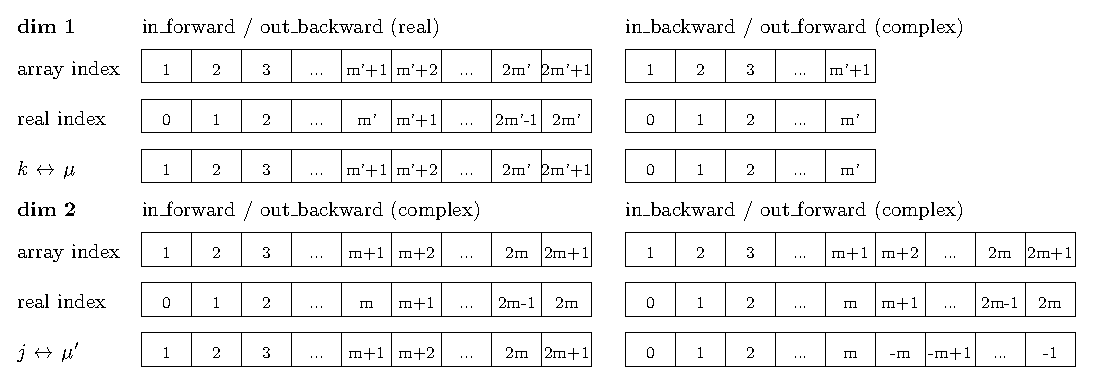
\includegraphics[width=1\textwidth]{_figure/fftw3_indices}
\par\end{center}

\caption[Indices arrangement in a complete forward-backward process of FFT-2D]{Indices arrangement in a complete forward-backward process of FFT-2D.
The DFT of dim 1 ($\Psi_{k}$ to $\mu$) and dim 2 ($\Phi_{k'}$ to
$\mu'$) are done consequentially and \emph{vice versa}. Array index
is the one of Fortran array, real index is the one shown in eq. (\ref{eq:fftw3-fwd})
and (\ref{eq:fftw3-bwd}), $k$ and $k'$ indices shown in the left
as well as $\mu$ and $\mu'$ in the right are those in eq. (\ref{eq:f_mup_mu})
and (\ref{eq:f_mup_mu_2}). Here $\mathrm{m}=m_{\mathrm{max}}$ and
$\mathrm{m}'=\left\lfloor m_{\mathrm{max}}/s\right\rfloor $. \label{fig:FFTW3-2D-indices}}
%
\end{minipage}
\end{figure}


\begin{figure}[h]
\centering{}%
\begin{minipage}[t]{1\textwidth}%
\begin{center}
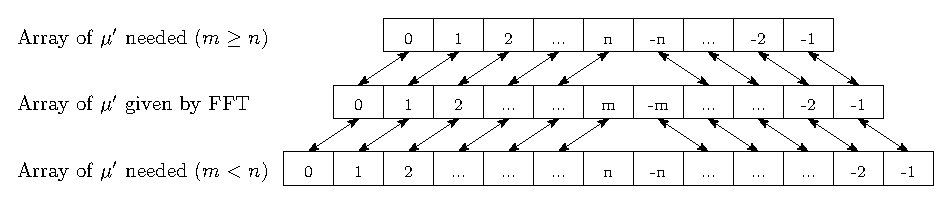
\includegraphics[width=1\textwidth]{_figure/mmax_to_nmax}
\par\end{center}

\caption[mmax to nmax]{mmax to nmax\label{fig:FFTW3-2D-mmax_to_nmax}}
%
\end{minipage}
\end{figure}


As the output array of FFTW3 is periodic
\begin{equation}
e^{2\pi i\mu k/n}=e^{2\pi i(\mu-n)k/n}e^{2\pi ik}=e^{2\pi i(\mu-n)k/n}\label{eq:mu-periodicity}
\end{equation}
the indices $\mu=m_{\mathrm{max}}+1,\ldots,2m_{\mathrm{max}}$ actually
corresponding to $\mu=-m_{\mathrm{max}},\ldots,-1$. It should be
noticed that eq. (\ref{eq:f_mup_mu}) and (\ref{eq:f_mup_mu_2}) don't
possess the periodicity of eq. (\ref{eq:mu-periodicity}), just in
the domain of definition of $\mu'$ and $\mu$ some intermediary functions
share the same formula with FFT.

Moreover, from eq. (\ref{eq:f_mup_mu}), (\ref{eq:f_mup_mu_3}) and
(\ref{eq:symm_f_m_mup_mu}) we can verify that
\begin{equation}
F_{\mu'\mu}(\Theta)=F_{-\mu',-\mu}^{*}(\Theta)
\end{equation}
The later is used in the code because according to the definition
in eq. (\ref{eq:fftw3-fwd}) and (\ref{eq:fftw3-bwd}), $F_{-\mu',-\mu}(\Theta)$
is calculated instead of $F_{\mu'\mu}(\Theta)$.


\section{Operational algorithm\label{sec:Operational-algorithm}}

As described above, the whole process of $\gamma$ and $\mathcal{F}_{\mathrm{exc}}$
functional evaluation is as shown: 

Firstly, the solvent density variable $\Delta\rho(\mathbf{r},\mathbf{\Omega})$
is expended on generalized spherical harmonics
\begin{equation}
\Delta\rho_{\mu'\mu}^{m}(\mathbf{r})=\frac{f_{m}}{8\pi^{2}}\int\mathrm{d}\mathbf{\Omega}\Delta\rho(\mathbf{r},\mathbf{\Omega})R_{\mu'\mu}^{m*}(\mathbf{\Omega})\label{eq:fgsht-fwd}
\end{equation}


Then the Fourier transform of these projections are computed
\begin{equation}
\Delta\hat{\rho}_{\mu'\mu}^{m}(\mathbf{k})=\int\mathrm{d}\mathbf{r}\Delta\rho_{\mu'\mu}^{m}(\mathbf{r})e^{-i\mathbf{r}\cdot\mathbf{k}}\label{eq:fft3d-fwd}
\end{equation}


Then the projections in k-frame are then rotated into local coordinates
system along the unit vector $\mathbf{\hat{k}}$
\begin{equation}
\Delta\hat{\rho'}_{\chi\mu}^{m}(\mathbf{k})=\sum_{\mu'}\Delta\hat{\rho}_{\mu'\mu}^{m}(\mathbf{k})R_{\mu'\chi}^{m}(\mathbf{\hat{k}})
\end{equation}
where the evaluation of rotation matrix elements by recurrence is
detailed \textcolor{red}{in appendix.}

Then computing the OZ equation with Blum's reduction
\begin{equation}
\hat{\gamma'}_{\chi\mu}^{m}(\mathbf{k})=\sum_{n,\nu}(-1)^{\chi+\nu}\hat{c}_{\mu\nu,\chi}^{mn}(\mathbf{k})\Delta\hat{\rho'}_{\chi\underline{\nu}}^{n}(\mathbf{k})\label{eq:OZ-2}
\end{equation}


Then the $\gamma$ projections are then transformed back to global
coordinates system
\begin{equation}
\hat{\gamma}_{\mu'\mu}^{m}(\mathbf{k})=\sum_{\chi}\hat{\gamma'}_{\chi\mu}^{m}(\mathbf{k})R_{\mu'\chi}^{m*}(\mathbf{\hat{k}})
\end{equation}


Then the inverse Fourier transform of these projections
\begin{equation}
\gamma_{\mu'\mu}^{m}(\mathbf{r})=\int\mathrm{d}\mathbf{k}\hat{\gamma}_{\mu'\mu}^{m}(\mathbf{k})e^{i\mathbf{r}\cdot\mathbf{k}}
\end{equation}


Then the function in angular frame can thus be rebuilt
\begin{equation}
\gamma(\mathbf{r},\mathbf{\Omega})=\sum_{m,\mu',\mu}f_{m}\gamma_{\mu'\mu}^{m}(\mathbf{r})R_{\mu'\mu}^{m}(\mathbf{\Omega})\label{eq:fgsht-bwd}
\end{equation}


Finally, the functional $\mathcal{F}_{\mathrm{exc}}$ is computed
by
\begin{equation}
\mathcal{F}_{\mathrm{exc}}=\frac{1}{2}\int\mathrm{d}\mathbf{r}\mathrm{d}\mathbf{\Omega}\Delta\rho(\mathbf{r},\mathbf{\Omega})\gamma(\mathbf{r},\mathbf{\Omega})
\end{equation}



\subsection{Reduction by symmetry\label{sub:Reduction-by-symmetry}}

A further reduction of computing cost can be made by performing approximately
only a half of operations, thanks to the symmetric relations between
the projections.

In eq. (\ref{eq:fgsht-fwd}), $\Delta\rho(\mathbf{r},\mathbf{\Omega})$
is real. Thanks to the property of GSH \textcolor{red}{(eq. (appendix))}
\[
R_{\mu'\mu}^{m}(\mathbf{\Omega})=(-)^{\mu'+\mu}R_{-\mu'-\mu}^{m*}(\mathbf{\Omega})
\]
we find
\begin{equation}
\Delta\hat{\rho}_{\mu'\mu}^{m}(\mathbf{r})=(-)^{\mu'+\mu}\Delta\hat{\rho}_{-\mu',-\mu}^{m*}(\mathbf{r})\label{eq:0}
\end{equation}
therefore only $\mu'>0$ or $\mu>0$ is needed to generate all information.

When $\Delta\hat{\rho}_{\mu'\mu}^{m}(\mathbf{r})$ is transformed
into $k$-space, replace eq. (\ref{eq:0}) into eq. (\ref{eq:fft3d-fwd})
gives
\begin{equation}
\Delta\hat{\rho}_{\mu'\mu}^{m}(\mathbf{k})=(-)^{\mu'+\mu}\Delta\hat{\rho}_{-\mu'-\mu}^{m*}(-\mathbf{k})\label{eq:1}
\end{equation}
thus only the projections of $\mu'>0$, $\mu>0$ or $\mathbf{k}$
where one of the dimensions $k_{i}>0$ are independent.

The rotation to local frame is reigned by the relation \textcolor{red}{(prove?)}
\begin{equation}
R_{\mu'\chi}^{m}(\hat{\mathbf{k}})=(-)^{m}R_{\mu',-\chi}^{m}(-\hat{\mathbf{k}})=(-)^{m+\mu'+\chi}R_{-\mu',\chi}^{m}(-\hat{\mathbf{k}})\label{eq:3}
\end{equation}
which gives
\begin{equation}
\Delta\hat{\rho'}_{\chi\mu}^{m}(\mathbf{k})=(-)^{m+\mu+\chi}\Delta\hat{\rho'}_{\chi,-\mu}^{m*}(-\mathbf{k})\label{eq:2}
\end{equation}
Thanks to the symmetry\textcolor{red}{{} (eq. (appendix))} 
\begin{equation}
\hat{c'}_{\mu\nu,\chi}^{mn}(k)=(-)^{m+n+\mu+\nu}\hat{c'}_{\underline{\mu}\underline{\nu},\chi}^{mn*}(k)
\end{equation}
\begin{equation}
\hat{c'}_{\mu\nu,\chi}^{mn}(k)=(-)^{m+n}\hat{c'}_{\nu\mu,\chi}^{nm}(k)
\end{equation}
\begin{equation}
\hat{c'}_{\mu\nu,\underline{\chi}}^{mn}(k)=\hat{c'}_{\underline{\mu}\underline{\nu},\chi}^{mn}(k)=(-)^{m+n}\hat{c'}_{\mu\nu,\chi}^{mn*}(k)
\end{equation}
$\hat{\gamma'}_{\chi\mu}^{m}(\mathbf{k})$ possesses the same symmetry.
Thus OZ equation can be reduced by a factor two.

\begin{figure}[h]
\begin{centering}
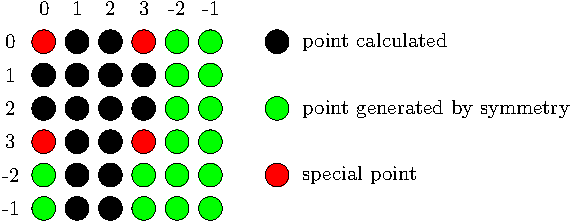
\includegraphics{_figure/test_lmn}
\par\end{centering}

\caption{Distribution of points to be calculated according to symmetry in a
2D plan}
\end{figure}



\subsection{Commutativity between operations\label{sub:Commutativity-between-operations}}

As mentioned in the operational algorithm, three types of operation
are being done before and after OZ equation. They are
\begin{enumerate}
\item Fast Fourier transform for 3-dimensional spatial grid (FFT3D): implemented
by package FFTW3 \citep{FFTW3}, mathematically leading to no accuracy
lost.
\item Fast generalized spherical harmonics transform (FGSHT): have real
or complex input, is exact if $F(\mathbf{\Omega})$ is a polynomial
of $\cos\Theta$, $\cos\Phi$ and $\cos\Psi$ of order at most $m_{\mathrm{max}}$.
\item Rotation between laboratory coordinate system and local system linked
to vector $\mathbf{k}$ (RotS): can be done for both function and
projections. It introduces a minus error in accuracy at origin and
border of the box, it will be discussed in next chapter.
\end{enumerate}
Their commutativity is shown in figure \ref{fig:Commutativity-of-operations}.

\begin{figure}[h]
\begin{centering}
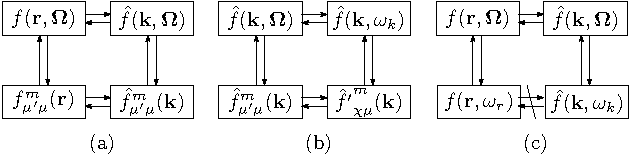
\includegraphics{_figure/algorithms_commutativity}
\par\end{centering}

\caption[Commutativity of operations]{Commutativity of operations. (a) FFT3D and FGSHT; (b) RotS and FGSHT;
(c) FFT3D and RotS\label{fig:Commutativity-of-operations}}
\end{figure}



\subsubsection{FFT3D and FGSHT}

The FFT3D

\[
f(\mathbf{r})=\int\hat{f}(\mathbf{k})e^{i\mathbf{k}\cdot\mathbf{r}}
\]
\[
\hat{f}(\mathbf{k})=\int f(\mathbf{r})e^{-i\mathbf{k}\cdot\mathbf{r}}
\]
does not depend on the angular part of function, and
\[
f(\mathbf{\Omega})=\sum_{m\mu'\mu}f_{m}f_{\mu'\mu}^{m}R_{\mu'\mu}^{m}(\mathbf{\Omega})
\]
\[
f_{\mu'\mu}^{m}=\int f_{m}f(\mathbf{\Omega})R_{\mu'\mu}^{m}(\mathbf{\Omega})
\]
does not depend on the spatial part of function. The two operations
are commutative.


\subsubsection{FGSHT and coordinate rotation}

Function $\hat{f'}$ intermolecular frame can be deduced from the
function $\hat{f}$ in laboratory frame 
\[
\hat{f}(\mathbf{k},\mathbf{\Omega})=\hat{f'}(\mathbf{k},\boldsymbol{\omega}_{k})
\]
where the two can both be expended on GSH

\[
\hat{f}(\mathbf{k},\mathbf{\Omega})=\sum_{m\mu'\mu}f_{m}\hat{f}_{\mu'\mu}^{m}(\mathbf{k})R_{\mu'\mu}^{m}(\mathbf{\Omega})
\]


\[
\hat{f'}(\mathbf{k},\boldsymbol{\omega}_{k})=\sum_{m\chi\mu}f_{m}\hat{f'}_{\chi\mu}^{m}(\mathbf{k})R_{\chi\mu}^{m}(\boldsymbol{\omega}_{k})
\]


And the relation between projections are simple

\[
f'{}_{\chi\mu}^{m}(\mathbf{k})=\sum_{\mu'}R_{\mu'\chi}^{m}(\hat{\mathbf{k}})f_{\mu'\mu}^{m}(\mathbf{k})
\]
\[
f_{\mu'\mu}^{m}(\mathbf{k})=\sum_{\chi}R_{\mu'\chi}^{m*}(\hat{\mathbf{k}})f'{}_{\chi\mu}^{m}(\mathbf{k})
\]
The two operations are commutative.


\subsubsection{Coordinate rotation and FFT3D}

The rotation from $f(\mathbf{r},\mathbf{\Omega})$ to $f(\mathbf{r},\boldsymbol{\omega})$
depends on the vector $\mathbf{r}$, of which the information is totally
lost after FFT3D. The rotation from $f(\mathbf{k},\mathbf{\Omega})$
to $f(\mathbf{k},\boldsymbol{\omega})$ can only depend on the vector
$\mathbf{k}$, they are not the same rotation. Non-commutative. 
